%===================================================================================
\section{Adjoint sensitivity analysis example problems}\label{s:adj_examples}
%===================================================================================

The next two sections describe in detail a serial example (\id{cvadx}) and
a parallel one (\id{pvanx}). For details on the other examples, the reader is
directed to the comments in their source files.

%------------------------------------------------------------------------
\subsection{A serial dense example: \id{cvadx}}\label{ss:cvadx}

As a first example of using {\cvodes} for adjoint sensitivity analysis
we examine the chemical kinetics problem of \S\ref{ss:serial_sim_ex} and
\S\ref{ss:serial_fwd_ex}:
\begin{equation}\label{e:chemkin:ivp}
  \begin{split}
    &{\dot y}_1 = -p_1 y_1 + p_2 y_2 y_3   \\
    &{\dot y}_2 =  p_1 y_1 - p_2 y_2 y_3 - p_3 y_2^2 \\
    &{\dot y}_3 =  p_3 y_2^2 \\
    &y(t_0) = y_0 \, ,
  \end{split}
\end{equation}
for which we want to compute the gradient with respect to $p$ of 
\begin{equation}\label{e:chemkin:G}
  G(p) = \int_{t_0}^{t_1}  y_3  dt ,
\end{equation}
without having to compute the solution sensitivities ${dy}/{dp}$.
Following the derivation of \S\ref{ss:adj_sensi} and taking into account
the fact that the initial values of (\ref{e:chemkin:ivp}) do not depend on 
the parameters $p$, by (\ref{e:dGdp}) this gradient is simply
\begin{equation}\label{e:chemkin:dGdp}
\frac{dG}{dp} = \int_{t_0}^{t_1} 
\left( g_p + \lambda^T f_p \right) dt \, ,
\end{equation}
where $g(t,y,p) = y_3$, $f$ is the vector valued function 
defining the right hand side of (\ref{e:chemkin:ivp}), and $\lambda$ is 
the solution of the adjoint problem (\ref{e:adj_eqns}),
\begin{equation}\label{e:chemkin:adj}
  \begin{split}
    &{\dot \lambda} = - (f_y)^T  \lambda - (g_y)^T \\
    &\lambda(t_1) = 0 \, .
  \end{split}
\end{equation}

In order to avoid saving intermediate $\lambda$ values just for the
evaluation of the integral in (\ref{e:chemkin:dGdp}), we extend the
backward problem with the following $N_p$ quadrature equations
\begin{equation}\label{e:chemkin:xi}
  \begin{split}
    &{\dot \xi} = g_p^T + f_p^T \lambda \\
    &\xi (t_1) = 0 \, ,
  \end{split}
\end{equation}
which yield $\xi(t_0) = - \int_{t_0}^{t_1} ( g_p^T + f_p^T \lambda) dt$
and thus ${dG}/{dp} = -\xi^T(t_0)$.
Similarly, the value of $G$ in (\ref{e:chemkin:G}) can be obtained as
$G = - \zeta(t_0)$, where $\zeta$ is solution of the following quadrature
equation:
\begin{equation}\label{e:chemkin:zeta}
  \begin{split}
    &{\dot\zeta} = g \\
    &\zeta(t_1) = 0 \, .
  \end{split}
\end{equation}

The source code for this example is listed in \A\ref{ss:cvadx}.
The main program and the user-defined routines are described below, 
with emphasis on the aspects particular to adjoint sensitivity calculations.
The calling program must include the {\cvodes} header file \id{cvodea.h} which
in turn includes \id{cvodes.h} and thus provides {\cvodes} function prototypes
and constants, including those in the adjoint sensitivity module.
 
This program also includes two user-defined accessor macros,
\id{Ith} and \id{IJth}
that are useful in writing the problem functions in a form closely
matching their mathematical description, i.e. with components numbered from 1 instead of from 0. 
Following that, the program defines problem-specific constants and a user-defined 
data structure which will be used to pass the values of the parameters $p$ to various
user routines. The constant \id{STEPS} defines the number of integration steps
between two consecutive check points.
The program prologue ends with the prototypes of four user-supplied functions that are
called by {\cvodes}. The first two provide the right hand side and dense Jacobian
for the forward problem and the last two provide the right hand side and dense Jacobian 
for the backward problem.

The \id{main} function begins with type declarations. Notice that we employ three vector
specification objects, \id{nvSpecF} for the forward problem, \id{nvSpecB} for
the adjoint problem, and \id{nvSpecQB} for the quadrature variables integrated on
the backward phase. The next code blocks allocate and initialize the user data
structure with the values of the parameters $p$, initialize \id{nvSpecF} by calling
the serial vector specification initialization routine from {\nvecs}, allocate and
initialize \id{y} with the initial conditions of the forward problem, and finally
set the tolerances \id{rtol} and \id{atol}.

The call to \id{CVodeCreate} creates the main integrator memory block for the 
forward integration and specifies the \id{BDF} integration method with \id{NEWTON} 
iteration. 
The next call specifies the optional user data pointer, while the call to \id{CVodeMalloc} 
sets-up the forward integration by specifying the intial conditions and integration 
tolerances. The linear solver is selected to be {\cvdense} through the call to its 
initialization routine \id{CVDense}. The user provided Jacobian routine \id{Jac}
and user data structure \id{data} are specified through calls to \id{CVDenseSetJacFn} and
\id{CVDenseSetJacData}, respectively.

Allocation for the memory block of the combined forward-backward problem is
acomplished through the call to \id{CVadjMalloc} which specifies \id{STEPS}=150,
the number of steps between two check points.

The call to \id{CVodeF} requests the solution of the forward problem to \id{TOUT}.
If successful, at the end of the integration, \id{CVodeF} will return the number
of saved check points in the argument \id{ncheck} (optionally, a list of the check points
can be printed by calling \id{CVadjCheckPointsList}).

The next segment of code deals with the setup of the backward problem. First,
a serial vector specification variable \id{nvSpecB} is initialized for vectors
of length \id{NEQ} (dimension of $\lambda$). A second serial
machine environmnet, \id{nvSpecQB} is initializaed for vectors of
dimension \id{NP+1} (dimension of $\xi$ $+$ one quadrature variable to evaluate $G$).
Following that, the program allocates space and initializes the variables of the 
backward problem and the relative and absolute tolerances for the backward integration.
{\cvodes} memory for the integration of the backward integration is created and allocated
by the calls to the interface routines \id{CVodeCreateB} amd \id{CVodeMallocB} which 
specify the \id{BDF} integration method with \id{NEWTON} iteration, among other things.
The dense linear solver {\cvdense} is then initialized by calling the \id{CVDenseB}
interface routine and specifying a non-\id{NULL} Jacobian routine \id{JacB} and user data
\id{data}.
Quadrature computation is initialized by calling \id{CVodeQuadMallocB}
which specifies the right hand side of the quadrature equations as \id{fQB} and tolerances
for the integration of quadrature variables.
The preceding call to \id{CVodeSetQuadErrConB} indicates that $\xi$ should not be considered 
in the error test.

The actual solution of the backward problem is acomplished through the call to
\id{CVodeB}. If successful, \id{CVodeB} returns the solution of the backward 
problem at time \id{T0} in the vector \id{yB}. The values of the quadrature
variables at time \id{T0} are loaded in \id{qB} by calling the extraction
routine \id{CVodeGetQuadB}. The values for $G$ and its gradient are printed next.

The main program continues with a call to \id{CVodeReInitB} and
\id{CVodeQuadReInitB} to reinitialize the 
backward memory block for a new adjoint computation with a different final 
time (\id{TB2}), followed by a second call to \id{CVodeB} and, upon successful
return, reporting of the new values for $G$ and its gradient.

The main program ends by freeing previously allocated memory through calls to 
\id{CVodeFree} (for the {\cvodes} memory for the forward problem), \id{CVadjFree} 
(for the memory allocated for the combined problem), \id{N\_VFree} 
(for the various vectors), and \id{NV\_SpecFree\_Serial} (for the three machine 
environment variables \id{nvSpecF}, \id{nvSpecB}, and \id{nvSpecQB}).

The user-supplied functions \id{f} and \id{Jac} for the right hand side and
Jacobian of the forward problem are straightforward expressions of its 
mathematical formulation (\ref{e:chemkin:ivp}), while \id{fB}, \id{fQB}, and \id{JacB}
are mere translations of the backward problem
(\ref{e:chemkin:adj})--(\ref{e:chemkin:xi})--(\ref{e:chemkin:zeta}).

The output generated by \id{cvadx} is shown below.

\vspace{0.1in}
\VerbatimInput[frame=single,framesep=0.1in,label={\tt cvadx} sample output,fontsize=\small]
{../examples_ser/cvadx.out}


%--------------------------------------------------------------------------

\subsection{A parallel nonstiff example: \id{pvanx}}
\label{ss:pvanx}

As an example of using the {\cvodes} adjoint sensitivity module with
the parallel vector module {\nvecp}, we describe a sample program
that solves the following problem: consider the 1-D advection-diffusion
equation
\begin{equation}\label{e:pvanx:orig_pde}
  \begin{split}
    & \frac{\partial u}{\partial t} = p_1 \frac{\partial^2 u}{\partial x^2} 
    + p_2 \frac{\partial u}{\partial x} \\
    & 0 = x_0 \le x \le x_1 = 2 \\
    & 0 = t_0 \le t \le t_1 = 2.5 \, ,
  \end{split}
\end{equation}
with boundary conditions $u(t,x_0) = u(t,x_1) = 0 ,\, \forall t$
and initial condition $u(t_0 , x) = u_0(x) = x(2-x)e^{2x}$. Also
consider the function
\begin{equation*}
  g(t) = \int_{x_0}^{x_1} u(t,x) dx \, .
\end{equation*}
We wish to find, through adjoint sensitivity analysis, the gradient of
$g(t_1)$ with respect to $p = [p_1 ; p_2]$ and the perturbation in $g(t_1)$
due to a perturbation $\delta u_0$ in $u_0$.

The approach we take in the program \id{pvanx} is to first derive an 
adjoint PDE which is then discretized in space and integrated backwards
in time to yield the desired sensitivities. A straight-forward extension 
to PDEs of the derivation given in \S\ref{ss:adj_sensi} gives
\begin{equation}\label{e:pvanx:dgdp}
  \frac{dg}{dp} (t_1) = \int_{t_0}^{t_1} dt 
  \int_{x_0}^{x_1} dx \mu \cdot 
  \left[
    \frac{\partial^2 u}{\partial x^2} ;
    \frac{\partial u}{\partial x}
  \right ]
\end{equation}
and
\begin{equation}\label{e:pvanx:delg}
  \delta g |_{t_1} = \int_{x_0}^{x_1} \mu(t_0,x) \delta u_0(x) dx \, , 
\end{equation}
where $\mu$ is the solution of the adjoint PDE
\begin{equation}\label{e:pvanx:adj_pde}
  \begin{split}
    & \frac{\partial \mu}{\partial t} + p_1 \frac{\partial^2 \mu}{\partial x^2} 
    - p_2 \frac{\partial \mu}{\partial x} = 0 \\
    & \mu(t_1 , x) = 1 \\
    & \mu(t , x_0) = \mu( t , x_1 ) = 0 \, .
  \end{split}
\end{equation}
Both the forward problem (\ref{e:pvanx:orig_pde}) and the backward problem 
(\ref{e:pvanx:adj_pde}) are discretized on a uniform spatial grid of size
$M_x + 2$ with central differencing and with boundary values eliminated,
leaving ODE systems of size $N = M_x$ each. 
As always, we deal with the time quadratures in (\ref{e:pvanx:dgdp}) by introducing
the additional equations
\begin{equation}\label{e:pvanx:quad}
  \begin{split}
    &{\dot\xi}_1 = \int_{x_0}^{x_1} dx \mu \frac{\partial^2 u}{\partial x^2} \, , \quad
    \xi_1(t_1) = 0 \, , \\
    &{\dot\xi}_2 = \int_{x_0}^{x_1} dx \mu \frac{\partial u}{\partial x} \, , \quad
    \xi_2(t_1) = 0 \, ,
  \end{split}
\end{equation}
yielding
\begin{equation*}
  \frac{dg}{dp} (t_1) = \left[ \xi_1(t_0) ; \xi_2(t_0) \right ]
\end{equation*}
The space integrals in (\ref{e:pvanx:delg}) and (\ref{e:pvanx:quad}) are
evaluated numerically, on the given spatial mesh, using the trapezoidal rule.

Note that $\mu(t_0 , x^*)$ is nothing but the perturbation in $g(t_1)$
due to a perturbation $\delta u_0(x) = \delta(x-x^*)$ in the initial conditions.
Therefore, $\mu(t_0,x)$ completely describes $\delta g(t_1)$ for any
perturbation $\delta u_0$.

The source code for this example is listed in \A\ref{ss:pvanx}. Both the forward
and the backward problems are solved with the option for nonstiff systems,
i.e. using the Adams method with functional iteration for the solution of
the nonlinear systems. The overall structure of the \id{main} function is very
similar to that of the code \id{cvadx} (\S\ref{ss:serial_adj_ex}) with 
differences arising from the use of the parallel vector module. Unlike 
\id{cvadx}, the example \id{pvanx} illustrates computation of the additional
quadrature variables by appending \id{NP} equations to the adjoint system.
This approach can be a better alternative to using special treatment
of the quadrature equations when their number is too small for parallel 
treatment.

Besides the parallelism implemented by {\cvodes} at the vector kernel level,
\id{pvanx} uses MPI calls to parallelize the calculations of the right-hand side
routines \id{f} and \id{fB} and of the spatial integrals involved.
The forward problem has size \id{NEQ = MX}, while the backward problem has
size \id{NB = NEQ + NP}, where \id{NP = 2} is the number of quadrature equations
in (\ref{e:pvanx:quad}).
The use of the total number of available processes on two problems of different 
sizes deserves some comments, as this is typical in adjoint sensitivity 
analysis. Out of the total number of available processes, namely \id{nprocs},
the first \id{npes = nprocs - 1} processes are dedicated to the integration of
the ODEs arising from the semi-discretization of the PDEs 
(\ref{e:pvanx:orig_pde}) and (\ref{e:pvanx:adj_pde}) and receive
the same load on both the forward and backward integration phases. 
The last process is reserved for the integration of the quadrature equations 
(\ref{e:pvanx:quad}), and is therefore inactive during the forward phases.
Of course, for problems involving a much larger number of quadrature equations,
more than one process could be reserved for their integration. 
An alternative would be to redistribute the \id{NB} backward problem variables 
over all available processes, without any relationship to the load distribution 
of the forward phase. However, the approach taken in \id{pvanx} has the 
advantage that the communication strategy adopted for the forward problem 
can be directly transfered to communication among the first \id{npes}
processes during the backward integration phase. 

We must also emphasize that, although inactive during the forward integration phase, 
the last process {\em must} participate in that phase with a 
{\em zero local array length}. 
This is because, during the backward integration phase, this process must
have its own local copy of variables (such as \id{cvadj\_mem}) that were set
only during the forward phase.

Sample output generated by \id{pvanx} is shown below.

\vspace{0.1in}
\VerbatimInput[frame=single,framesep=0.1in,label={\tt pvanx} sample output,fontsize=\small]
{../examples_par/pvanx.out}


%--------------------------------------------------------------------------

\subsection{An SPGMR parallel example using the CVBBDPRE module: \id{pvakx}}
\label{ss:pvakx}

\begin{figure}
  {\centerline{\psfig{figure=pvakx2D.eps,width=\textwidth}}}
  \caption[Results for the \id{pvakx} example problem in 2D.]
  {Results for the \id{pvakx} example problem in 2D. 
    The gradient with respect to the source parameters is pictured on the left. 
    On the right, the gradient was color coded and superimposed over the nominal value 
    of the source parameters.}
  \label{f:pvakx2D}
\end{figure}

\begin{figure}
  \begin{center}
    \mbox{
      \subfigure[Nominal values of the source parameters.]
      {\includegraphics[width=0.75\textwidth]{pvakx3Dcf.eps}}
    }
    \mbox{
      \subfigure[Two isosurfaces of the gradient with respect to the source parameters.
      They correspond to values of $0.25$ (green) and $0.4$ (blue).]
      {\includegraphics[width=0.75\textwidth]{pvakx3Dgrad.eps}}
    }
  \end{center}
  \caption{Results for the \id{pvakx} example problem in 3D.}
  \label{f:pvakx3D}
\end{figure}

A sample output generated by \id{pvakx} for a 2D calculation is shown below.

\vspace{0.1in}
\VerbatimInput[frame=single,framesep=0.1in,label={\tt pvakx} sample output,fontsize=\small]
{../examples_par/pvakx.out}

